% !TeX spellcheck=en_GB
\documentclass{beamer}
%\documentclass[handout]{beamer}
\usepackage{etex}
%% % use this with the [handout] option to create handouts for the audience
% \usepackage{pgfpages}
% \pgfpagesuselayout{2 on 1}[a4paper,border shrink=5mm]

\mode<presentation>
{
  \usetheme{Diku}
  % set this to your preferences:
  \setbeamercovered{invisible}
  %\setbeamercovered{transparent}
}
\usepackage{listings}
\usepackage{framed}
\usepackage{graphicx}
\usepackage{adjustbox}
\usepackage{epic}
\usepackage{url}
\usepackage{paratype}
\usepackage{xcolor}
\usepackage{ulem}
\usepackage{multirow}
\usepackage[utf8]{inputenc}
\usepackage{caption}
\usepackage{mathrsfs}
\setbeamerfont{frametitle}{family=\bf}


\setbeamertemplate{bibliography item}{\insertbiblabel}

\usepackage{amsmath}
\usepackage{amssymb}
\usepackage{amsthm}

\newcommand{\basetop}[1]{\vtop{\vskip-1ex\hbox{#1}}}
\newcommand{\source}[1]{\let\thefootnote\relax\footnotetext{\scriptsize\textcolor{kugray1}{Source: #1}}}
\definecolor{mygreen}{RGB}{50, 96, 60}

\lstdefinelanguage{Futhark}
{keywords={fun,if,then,else,loop,do,map,reduce,filter,scan,redomap,transpose,reshape,iota,replicate,let,in,for,while,with,f32,int,zip,streamRed,zipWith, unsafe, done, return},% done,return is a hack <- pseudocode not futhark
  sensitive=true,%
  comment=[l]{--},%
  string=[b]",%
  moredelim=**[is][\color{red}]{@}{@},
  moredelim=**[is][\color{structure}]{¤}{¤},
}

\lstset{
  language=Futhark,
  basicstyle=\footnotesize
}

% for coloured code citation in text:
\usepackage{fancyvrb}

%%%%%%%%%%%%%%%%%%%%%%%%%%%%%%%%%
%%%%% code sections   %%%%%%%%
%%%%%%%%%%%%%%%%%%%%%%%%%%%%%%%%%

% code highlighting commands in own block
\DefineVerbatimEnvironment{code}{BVerbatim}{}
\DefineVerbatimEnvironment{icode}{Verbatim}{fontsize=\scriptsize}
\DefineVerbatimEnvironment{tinycode}{Verbatim}{fontsize=\tiny}

% Fancy code with color commands:
\DefineVerbatimEnvironment{colorcode}%
{Verbatim}{fontsize=\scriptsize,commandchars=\\\{\}}
\DefineVerbatimEnvironment{smallcode}%
{Verbatim}{fontsize=\tiny,commandchars=\\\{\}}

%%%%%%%%%%%%%%%%%%%%%%%%%%%%%%%%%%
%%%%% some coloring    %%%%%%%%

% use "DIKU green" from our color theme for \emph
\renewcommand{\emph}[1]{\textcolor{structure}{#1}}
% use some not-too-bright red for an \emp command
\definecolor{DikuRed}{RGB}{130,50,32}
\newcommand{\emp}[1]{\textcolor{DikuRed}{ #1}}
\definecolor{CosGreen}{RGB}{10,100,70}
\newcommand{\emphh}[1]{\textcolor{CosGreen}{ #1}}
\definecolor{CosBlue}{RGB}{55,111,122}
\newcommand{\emphb}[1]{\textcolor{CosBlue}{ #1}}
\definecolor{CosRed}{RGB}{253,1,1}
\newcommand{\empr}[1]{\textcolor{CosRed}{ #1}}

\newcommand{\mymath}[1]{$ #1 $}
\newcommand{\myindx}[1]{_{#1}}
\newcommand{\myindu}[1]{^{#1}}

\newcommand{\myalt}{~|~}

\makeatletter
\long\def\beamer@author[#1]#2{%
  \def\insertauthor{\def\inst{\beamer@insttitle}\def\and{\beamer@andtitle}%
    \begin{tabular}{lr}#2\end{tabular}}%
  \def\beamer@shortauthor{#1}%
  \ifbeamer@autopdfinfo%
  \def\beamer@andstripped{}%
  \beamer@stripands#1 \and\relax
  {\let\inst=\@gobble\let\thanks=\@gobble\def\and{, }\hypersetup{pdfauthor={\beamer@andstripped}}}
  \fi%
}
\makeatother

%%%%%%%%%%%%%%%%%%%%

\title{Programming Massively Parallel Hardware\\\textbf{Simplex on the GPU}}

\author[]{%
  Anders Wind Steffensen \\
  Chi Pham \\
  Michael Hejselbak Jensen \\
}

\institute{Department of Computer Science (DIKU)\\University of Copenhagen}


\date[3/3]{November 9th 2017}


\begin{document}

\titleslide

%%%%%%%%%%%%%%%%%%%%%%%%%%%%%%%%%%%%%%%%%%%%%%%%%%%%%%%%%%%%%%%%%%%%%%

\begin{frame}
  \frametitle{Overview}
  \begin{itemize}
  \item Introduction
  \item Design
  \item Experiments
  \item Results
  \item Conclusion
  \end{itemize}
\end{frame}

%%%%%%%%%%%%%%
% INTRO
%%%%%%%%%%%%%%

\begin{frame}
\frametitle{Introduction}
\framesubtitle{Motivation}
\centering
{\Large What problem are we trying to solve?}

\begin{itemize}
	\item Linear programming models optimisation problems.
	\item Simplex is an algorithm for solving linear programs.
	\item There have been attempts to parallelise Simplex ...
	\pause
	\item ... but never across multiple linear programs. {\tiny (to our knowledge)}
\end{itemize}
\end{frame}

\begin{frame}
\frametitle{Introduction}
\framesubtitle{Focus}
\centering
{\Large What is the scope of this project?}

\begin{itemize}
\item Implement parallel versions of Simplex.
\item Experiment with parallelism across multiple dimensions.
\item Benchmark our programs and compare with 'state of the art' implementation, CPLEX.
\end{itemize}
\end{frame}

\begin{frame}[fragile]
\frametitle{Introduction}
\framesubtitle{Simplex}
\centering
{\Large What does Simplex do?}

\begin{itemize}
\item Goal is to optimise a linear function of $n$ variables, subject to $m$ linear constraints.
\item Simplex consists of a convergence loop in which we \emph{pivot}.
\item The \emph{pivot} updates an $m \times n$ matrix $A$, an $m$-vector $b$, and an $n$-vector $c$.
\item Number of pivots before convergence is worst case exponential.
\end{itemize}
\end{frame}

%%%%%%%%%%%%%%
% DESIGN
%%%%%%%%%%%%%%

\begin{frame}[fragile]
\frametitle{Design}
\framesubtitle{Multi-Simplex}
\begin{lstlisting}
Entering-Variable(c[n]) = ¤reduce, iota¤
Leaving-Variable(A[m][n], b[m], e) = ¤map, reduce, iota¤
Pivot(A[m][n], b[m], c[n], v, e, l) = ¤map, iota¤

Simplex(A[m][n], b[m], c[n]) =
  v = 0
  e = Entering-Variable(c)
  while (e != -1) do
    ¤l = Leaving-Variable(A,b,e)
    (A,b,c,v) = Pivot(A,b,c,v,e,l)
    e = Entering-Variable(c)¤
  done
  return v
\end{lstlisting}
\pause
\begin{lstlisting}
Multi-Simplex(As[h][m][n], bs[h][m], cs[h][n]) =
  map Simplex As bs cs
\end{lstlisting}
\empr{Amortise convergence loop across multiple instances!}
\end{frame}

\begin{frame}
\frametitle{Design}
\framesubtitle{Implementations}
\begin{itemize}
	\item \textbf{Outer parallel}: Instances are computed in parallel. Simplex is not parallelized. Flattening is not needed.
	
	\item \textbf{Inner parallel}: Simplex is computed in parallel. Not parallel across instances. Small degree of flattening.
	
	\item \textbf{Fully parallel}: Simplex and instances are computed in parallel. High degree of flattening.
\end{itemize}
\end{frame}

\begin{frame}
\frametitle{Design}
\framesubtitle{Limitations and obstacles}
\begin{itemize}
	\item The sequential convergence loop is the hard limit on achievable speed-up. Worst case exponential. 
	
	\item Flattening overhead inside convergence loop.
	
	\item Low level of thread utilization when number of pivots differ across instances.
\end{itemize}
\end{frame}

\begin{frame}
\frametitle{Design}
\framesubtitle{Observations}
\begin{itemize}
	\item The convergence loop gets amortized over the number of instances.
	
	\item Iota is amortized over the convergence loop since it can be hoisted outside.
	
	\item Each pivot is then only map operations, minimizing synchronization and work depth.
\end{itemize}
\end{frame}

%%%%%%%%%%%%%%
% IMPLEMENTATION
%%%%%%%%%%%%%%

\begin{frame}
	\frametitle{Experiments}
	\framesubtitle{Test generation}
	\begin{itemize}
		\item Parametrized on \#instances, \#variables, \#constraints. Fixed range of random values
		
		\item Each parameter affects the running time significantly. The significance of values is not immediately obvious.
		
		\item Superfluous constraints and variables.
	\end{itemize}
\end{frame}

\begin{frame}
\frametitle{Experiments}
\framesubtitle{Benchmark categories}
\begin{itemize}
	\item \textbf{One Big Instance}: benchmarks the implementations performance of Simplex.
	
	\item \textbf{Many Small Instances}: benchmarks the implementations performance of running Simplex many times where each computation of Simplex is diminished.
	
	\item \textbf{Many Big Instances}: benchmarks the implementations performance of running Simplex many times where each iteration of Simplex is significant.
	
	\item \textbf{Many Varying Instances}: benchmarks the implementations performance of running Simplex over many instances where Simplex might or might not be significant.
\end{itemize}
\end{frame}

%%%%%%%%%%%%%%
% RESULTS
%%%%%%%%%%%%%%
\begin{frame}[fragile]
\frametitle{Results}
\framesubtitle{One Big Instance}
\centering
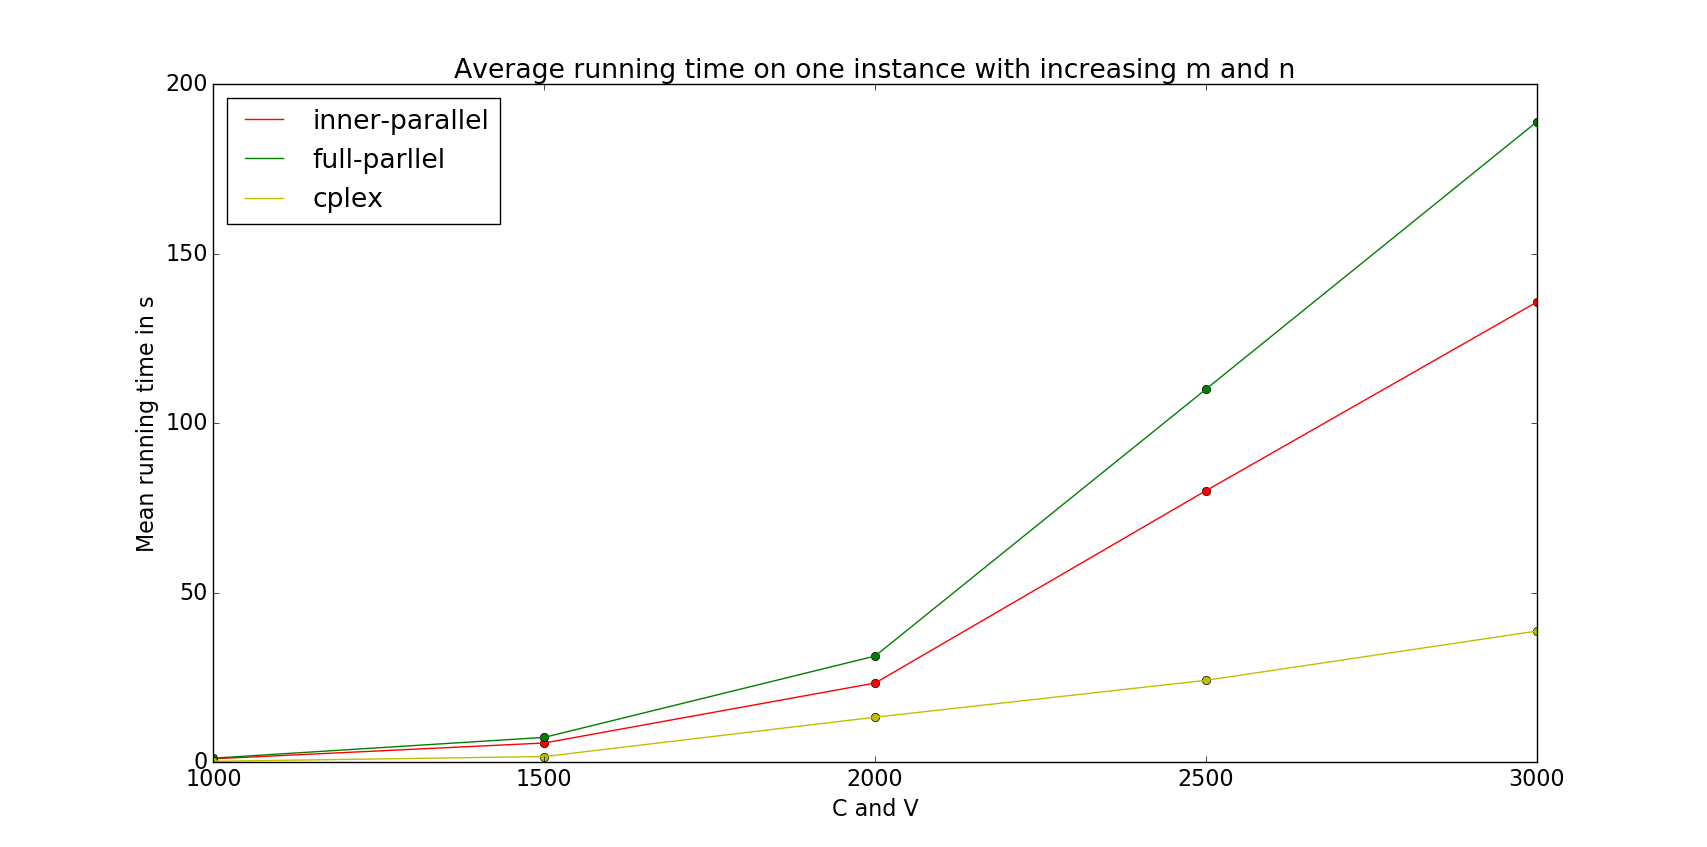
\includegraphics[width=0.9\textwidth]{../Doc/figures/one-big-new}
\begin{itemize}
	\item Inner parallel $\sim$23 times faster than sequential (not on graph).
	\item Fully parallel is slightly slower than inner.
	\item CPLEX algorithmic optimizations.
\end{itemize}
\end{frame}

\begin{frame}[fragile]
\frametitle{Results}
\framesubtitle{Many Small Instances}
\centering
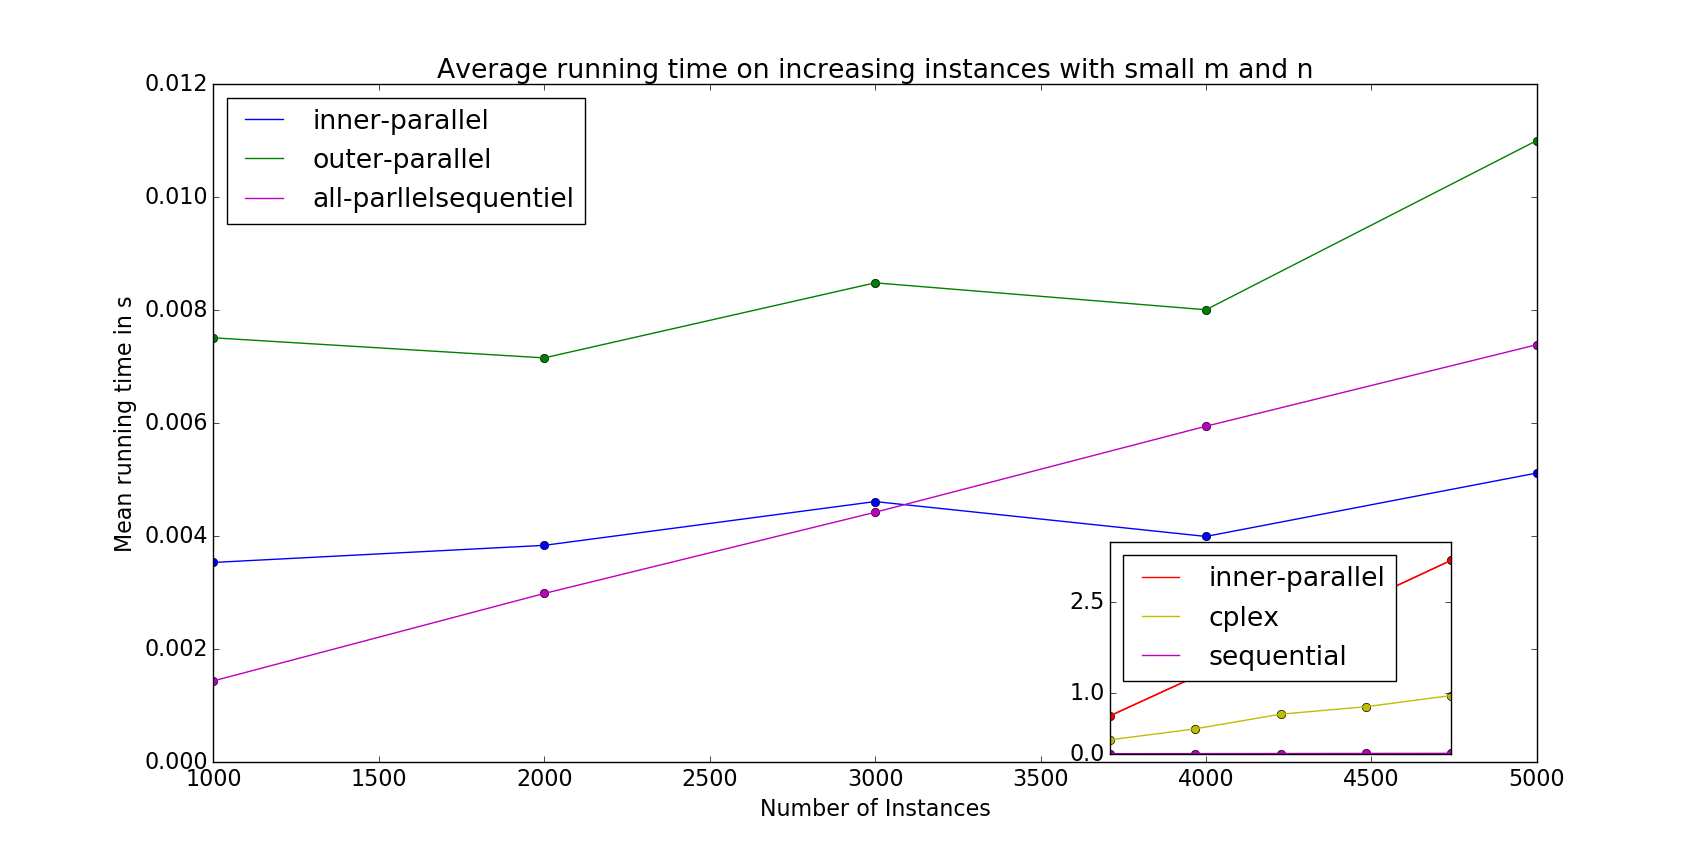
\includegraphics[width=0.85\textwidth]{../Doc/figures/many-small-in-one}
\begin{itemize}
	\item Outer parallel only faster than sequential for high number of instances - overhead for starting each instance is significant.
	\item Calculation of simplex is more important than parallelization across instances.
	\item CPLEX not optimized for solving multiple instances. Outer parallel $\sim$188 times speed-up.
\end{itemize}
\end{frame}

\begin{frame}[fragile]
\frametitle{Results}
\framesubtitle{Many Big Instances}
\centering
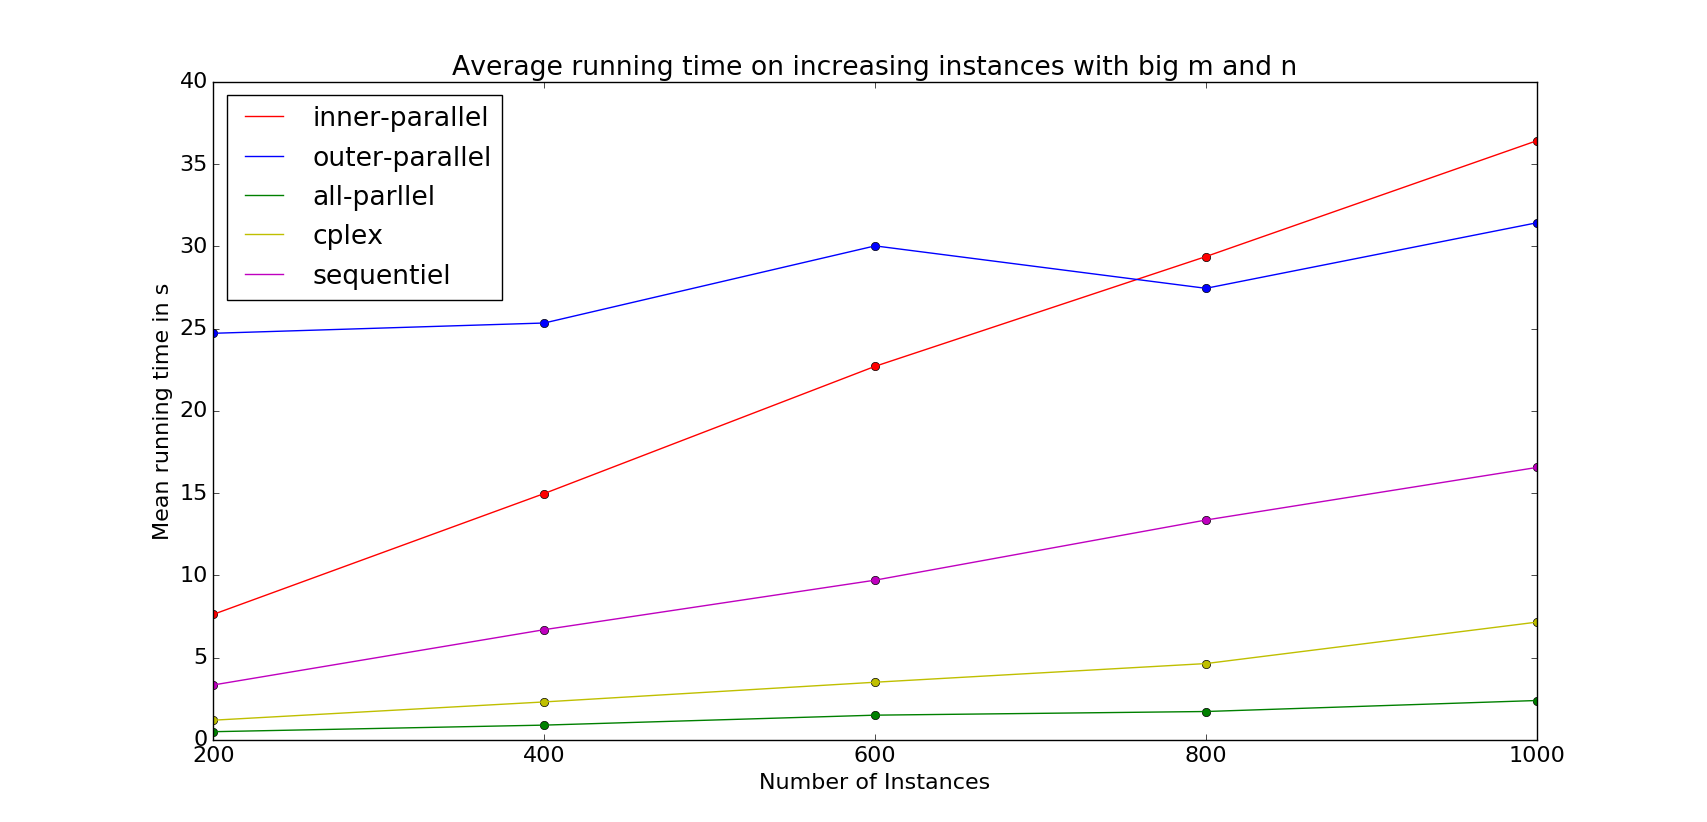
\includegraphics[width=0.9\textwidth]{../Doc/figures/many-big}
\begin{itemize}
	\item Fully parallel $\sim$7 times faster than sequential and $\sim$3 times faster than CPLEX.
	\item Sequential is faster than both inner and outer.
	\item Outer scales better than inner.
\end{itemize}
\end{frame}

\begin{frame}[fragile]
\frametitle{Results}
\framesubtitle{Many Instances of Varying Size}
\centering
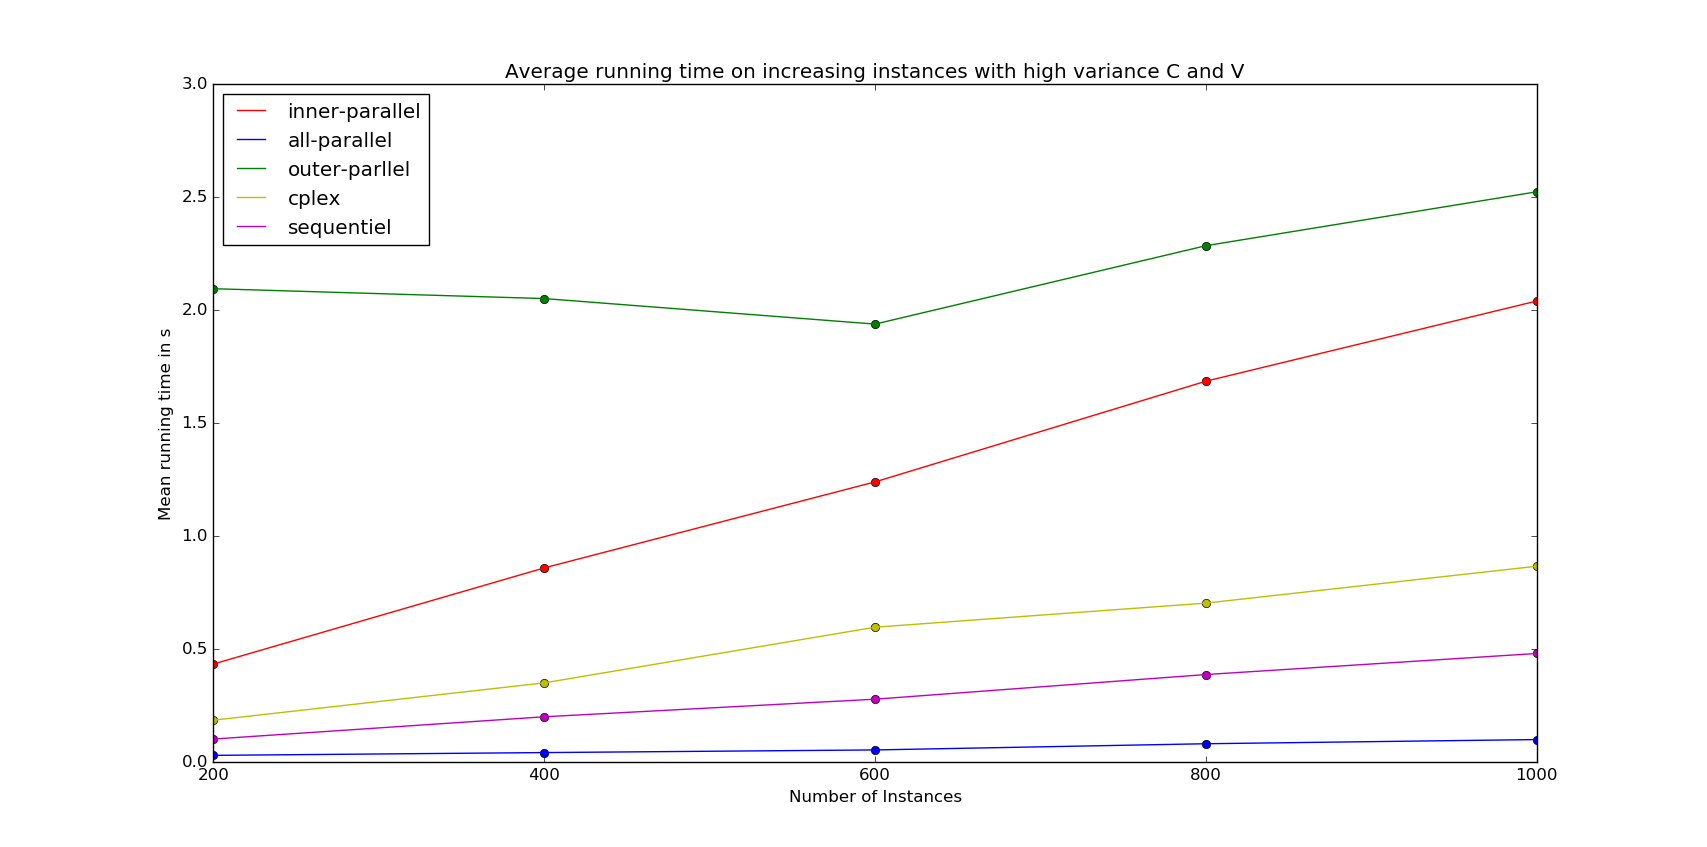
\includegraphics[width=0.9\textwidth]{../Doc/figures/many-varying}
\begin{itemize}
	\item Fully parallel $\sim$8 times faster than sequential and $\sim$4.5 times faster than CPLEX.
	\item Fully parallel scales really well.
\end{itemize}
\end{frame}

\begin{frame}
\frametitle{Results}
\framesubtitle{Evaluation}
\centering
{\Large What did we learn?}

\begin{itemize}
\item Fully parallel combines best of inner and outer parallel.
\item Fully parallel overhead is negligible compared to inner and outer.
\pause
\item Convergence loop is huge bottleneck.
\item Instance size is more significant than \# instances
\item CPLEX scales much better with instance size.
\end{itemize}

%For extreme cases, we have inner and outer perform best. But they are terrible when their own parallel dimension is not used. Fully parallel is never far behind and works well on both extremes. EXCEPT for one big.
\end{frame}

\begin{frame}
\frametitle{Results}
\framesubtitle{Improving the Results}
If the convergence loop is our bottleneck, what can we do?

\begin{itemize}
\item Decrease overhead of an iteration {\tiny($\leftarrow$ CPLEX, probably)}
\item Decrease number of iterations {\tiny($\leftarrow$ also CPLEX)}
\end{itemize}

\pause
How many iterations are actually needed?
\begin{figure}
\begin{tabular}{|c|c|c|c|c|}
\hline
\emph{\textbf{Number of instances}} & \emph{\textbf{Size range}} & \emph{\textbf{Mean iterations}} & \emph{\textbf{Std.}} \\\hline
5000 & 1-10 & $\sim 4$ & $\sim 3$ \\\hline
3000 & 10-150 & $\sim 77$ & $\sim 54$ \\\hline
1000 & 150-200 & $\sim 254$ & $\sim 80$ \\\hline
1 & 5000 & 57994 & 0 \\\hline
\end{tabular}
\end{figure}
\end{frame}

\begin{frame}[fragile]
\frametitle{Results}
\framesubtitle{Improving the Results}
\centering
Futhark uses \texttt{memcpy} in each loop iteration.

An experiment: unroll loop to decrease number of \texttt{memcpy}'s.

\pause

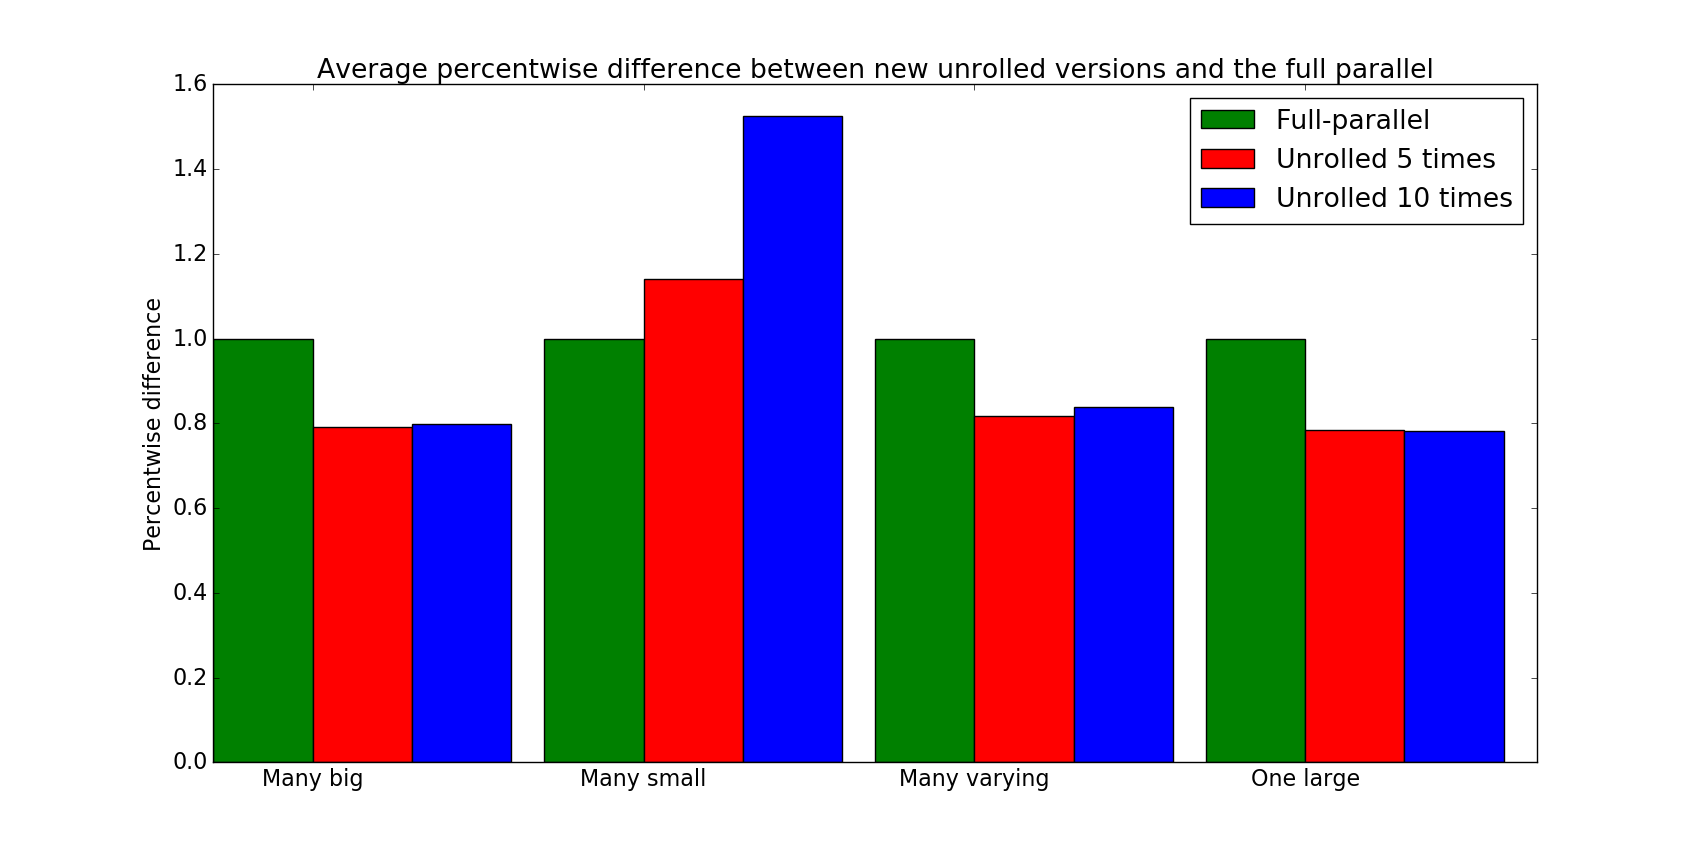
\includegraphics[width=0.9\textwidth]{../Doc/figures/unrolling}

 \empr{Result: 20\% faster when unrolling 5 iterations! {\tiny(for big enough instances)}}

\end{frame}


%%%%%%%%%%%%%%
% CONCLUSION
%%%%%%%%%%%%%%

\begin{frame}
\frametitle{Conclusion}
\framesubtitle{Further Work}
\begin{itemize}
	\item Experiment to clarify for what sizes and what number of instances the fully parallel does better than CPLEX.
	\item Preprocessing to decrease size and number of iterations
	\item Better rules for finding entering and leaving variable. Compute multiple pivots from same basis in parallel and pick best.
	\item Implement fully parallel versions of other types of Linear Programming algorithms.
	\item Investigate Futhark implementation to identify spots with unnecessary overhead (e.g. data copying).
\end{itemize}
\end{frame}

\begin{frame}
\frametitle{Conclusion}
\begin{itemize}
	\item We implemented a parallel version which is faster than the state of the art framework when the the number of instances outweighs the sizes of the instances.
	\item The cost of flattening is minimal compared to the ability to scale well on both \# instances and the instance sizes.
	\item A lot of possible further research.
\end{itemize}
\end{frame}

\end{document}
